%!TEX root = ../Thesis.tex
\chapter{Predict permeation enhancement}

A main goal of this thesis has been to use the preclinical data more efficiently. Instead of testing randomly new absorption enhancers or what intuitively seems promising, a model built on previous experiences, can swiftly evaluate larger libraries of molecules.

\subsection{Work flow and early challenges}
\label{predPerm:workflow}

Very early in the project three areas to predicts were identified. These were solubility, critical micelle concentration (CMC) and permeation enhancement. In Novo Nordisk for purposes securing intellectual properties, the default rule is that no in-house data generated by the drug development projects can be published. Therefore all data used in this PhD thesis were already public available from third-party sources or conducted in experiments for this thesis only.

Figure \ref{predict_workflow} outlines the work flow of establishing a model to predict permeation enhancement.

\begin{figure}[!htbp]

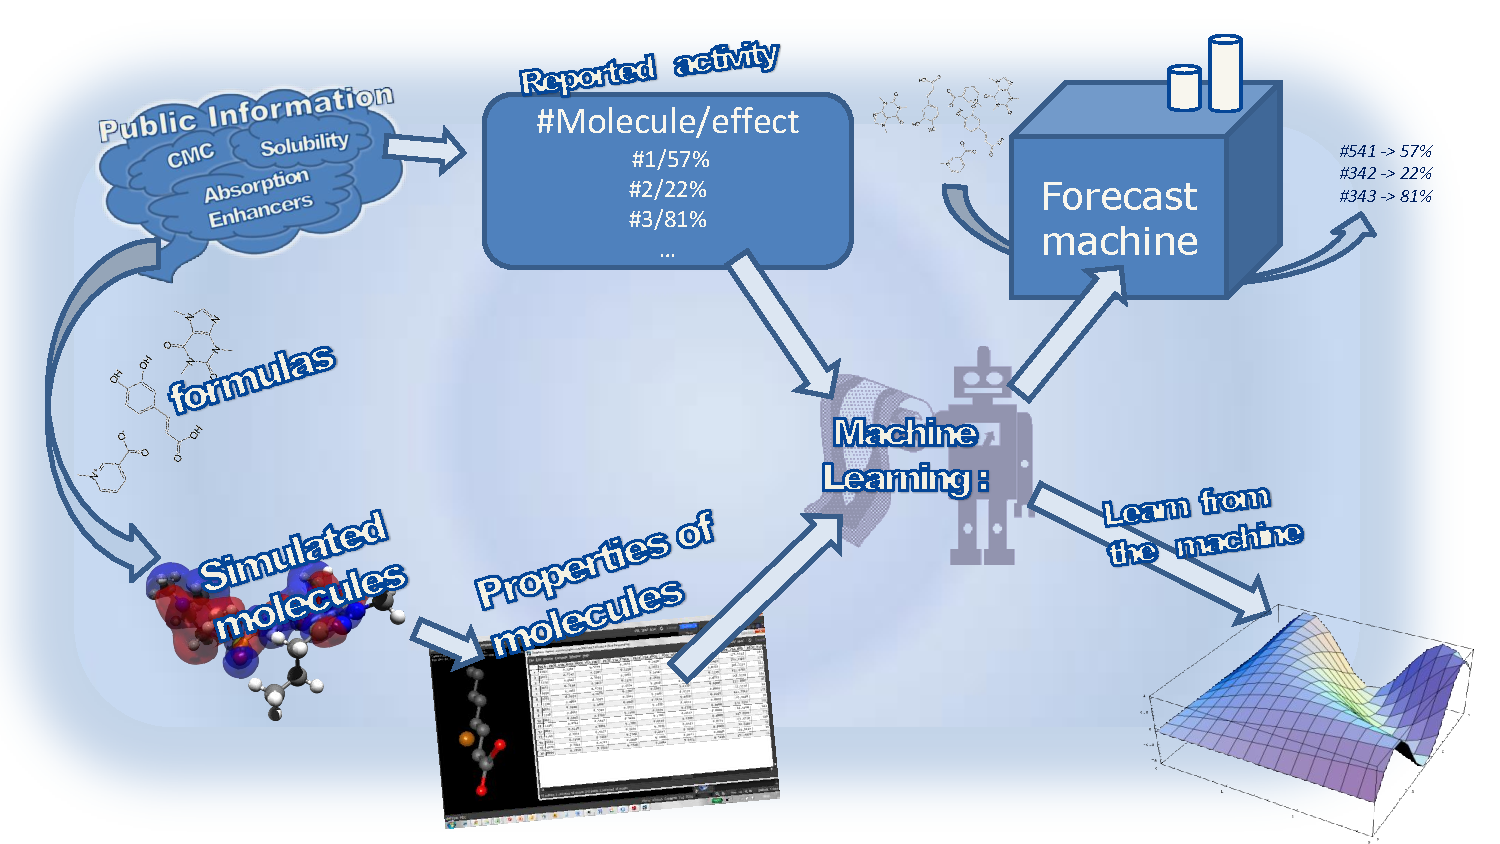
\includegraphics[width=\textwidth, height=\textheight, keepaspectratio]{graphics/predictPotencySummary.pdf}
\caption{Public information are tables of measured activity (target) linked to unique molecule formulas. Formulas of molecules can be simulated with e.g. force field models to extract calculated properties (features / descriptors). A machine learning algorithm uses target and features to output a model. The model is used as a forecast machine, and the model can be inspected to learn from the machine.}
\label{predict_workflow}
\end{figure}

The work flow outlines a bottom up approach, where very simple \textit{in-vitro} experiments are conducted for series of candidate molecules. Each molecular formula is first characterized by external models simulating the molecule and calculating molecular descriptors, see Section \ref{modelMolecules} and the methods part 3.2 of article in Section \ref{article:predAbs}. A relationship is established with the learning algorithm between the molecular formula and the \textit{in-vitro} response.

Data on \textit{in-vitro} Caco-2 permeation enhancement or similar preclinical studies were not expected alone to be useful to select new enhancers. In-vitro studies tend to overestimate the importance and impact of lipophilicity and the overall effect of absorption enhancer. Enhancers with C16 carbon chains are found 10-50 fold more potent than their C10 counter parts. \cite{maher2009safety,tippin2008biorelevant}. Nevertheless C16 carbon chain based permeation enhancer, have quite disappointing not delivered the same potency in \textit{in-vivo} studies. An obvious testimony is that there is no public announced clincal trials using C16 surfactant peptide absorption enhancers \cite{aguirre2016current}.

A starting project hypothesis was, that critical micelle concentration (CMC) was correlated with high absorption potency. Therefore initially, to collect data sets on CMC values was a central goal. Being able to predict CMC could assist the selection of permeation enhancer candidates. However, I found no literature that in fact shows, that low CMC values directly should cause permeation enhancement. Rather CMC is simply being one of more collective attributes associated with lipophilicity \cite{rosen2012surfactants}. Surfactants can be effective below their CMC \cite{xia2000mechanistic}. Therefore, it would make more sense to build predictive model using a target that resembled the permeation enhancement the most. Therefore Caco-2 measurements was finally favored over CMC measurements as model target.

Molecular solubility in watery buffers is not surprisingly negatively associated with lipophilicity / hydrophibicity. In a worst case scenario potency predictions and solubility predictions would be highly negatively correlated. Then to the models, permeation potency and in-solubility would be two indistinguishable phenomena. Such a failure of the model destinguish insolubility with permeation enhancement would contract the observed population of permeation enhancers in litterature, as elongating the carbon chain of any molecule making it more lipophile, does not necessarily make a potent permeation enhancer. In the article of Section \ref{article:predAbs}, I used an early version of the developed random forest diagnostic package forestFloor \cite{welling2016forest}, to discover that the trained permeation enhancement model in fact had captured this distinction in an interaction term. See Section \ref{defineInteractions} of how I define and classify interactions for non-linear models such as random forest.

\subsection{Challenges of a top down modeling of permeation enhancement}
In opposite to the bottom up approac of modeling simplified \textit{in-vitro} experiments, a top down approach was also being followed early in the project. Hypothesis associated with top down approach was, that molecules claimed in literature such as articles and patent applications to be permeation enhancers could be used as training examples.

One data set was obtained in an effort to use text mining to collect examples of compounds being mentioned for being permeation enhancers and/or absorption enhancers. The data set was acquired as a part of Sarah Brebbia Dirksen (Øster) master thesis project in 2012. A list of 167 compounds originating from patent applications and research articles was compiled \cite{sara2012application}.

Such a set of examples would not only reflect \textit{in-vitro} studies, but also a series of unknown limitations such as toxicology, formulation in-capabilities etc. Thus a model build on target data in the end stage of process, may contain a number of favorable biases, such that the model e.g. tend not to suggest toxic molecules as permeation enhancers.

It was assumed that permeation enhancement is a rare property of molecules, such that any random molecule would likely not be an enhancer. Random molecules of similar weight was acquired with the software ACDlab. Hereafter 49 chemical descriptors were computed for both sets of molecules using the software packages ACDlabs and Molecular operating environment (MOE). Linear discriminant analysis has been used to learn a class separation rule to identify typical enhancer like molecules \cite{sara2012application}.

Although a valid cross-validation of the classification model predicted a nearly perfect classification accuracy, the model failed in a proof of concept to test predicted molecules in-house in the Caco-2 model. There are a number reasons why this approach can have failed in spite of a promising cross-validation. To be fair some of these reasons were discussed in the fine master thesis of \cite{sara2012application}. However, in the clear light of hind sight, let us in the following section evaluate the implicit assumptions of this top-down approach.

\subsection{Assumptions of the top-down model}
A requirement was that training and future test observations had to be drawn from same distributions, see Section \ref{iid}. The training set originated with positive examples from the pharmaceutical literature and with negative examples from what appeared to be a random synthesis chemical library. It was assumed that all molecules from random synthesis library were not effective as enhancers, and  I agree on this as a fair assumption. However visually inspecting the random synthesis molecules, revealed these molecules were far from typical excipients of pharmaceutical formulations. Exotic heavy atoms as uranium! or what appear to be a truly random patterns of side group substitutions was observed. If this library in fact was generated as an random or an exhaustive search of possible molecule graphs below a given molar weight, then the average molecules will look far from the typical excipients as these are certainly not random molecules for a number of reasons. The typical excipient, especially surfactant enhancers, are not very substituted, not very branched. If generating a molecule starting from one carbon atom, and any choice has equal probability, should this carbon chain branch out here or not? Should there be substituted something here or not? The average molecule will be very branched and highly substituted, simply because there the combinatorial space is bigger, than for non-branched non-substituted carbon chains. Thus the classification model has been trained to recognize the difference between two groups of molecule that are obviously different. A part of the reason the two classes of molecules are different may well properties related to being permeation enhancers or not. However any other differences between the groups will be confounded permeation enhancement.

Most likely such classification model would be used to scan through a library of approved pharmaceutical excipients, thus only drawing observations to predict from the pharmaceutical molecule distribution. Suddenly the model may recognize many of the molecules as permeation enhancers, simply because these are not branched enough or highly substituted. The model will suggest too many molecules as permeation enhancers and not all can be tested. One could use the linear discriminant score to rank the predicted molecules to select those, who where most likely permeation enhancers. However classic linear discriminant analysis, do not employ a proper score function such as the breier score and is not calibrated to rank how likely predicted molecules are permeation enhancers.

Supervised machine learning is based rely on, that proximate observations have similar targets on the smallest scale in the feature space, such that some interpolation is a meaningful prediction. However, if including receptor mediated permeation enhancers or calcium chelators. Receptor-agonist interactions are very delicate processes that in two ways are analogous to a lock and key. First a permeation enhancer agonist will like a key fit in a membrane receptor lock and trigger a response. Secondly, just the slightest change of the key or lock could disable the activation. To map any possible key combination would take a very high number of training examples. Likewise for receptor mediated permeation enhancers or calcium chelators, just a single reconfiguration of an atom, could completely change the biological response. A few hundred molecules mentioned in litterature is likely very far from mapping the entire complex mechanism of a living cell. In contrary surfactant-like permeation enhancers will likely to some extend elicit their effect through surface tension depression. A single atom reconfiguration will likely not completely revert the physiochemical properties and an interpolation on the small scale will be meaning full.

\subsection{orphan! figure explaining why in-vitro studies over estimate}
\begin{figure}[!htpb]
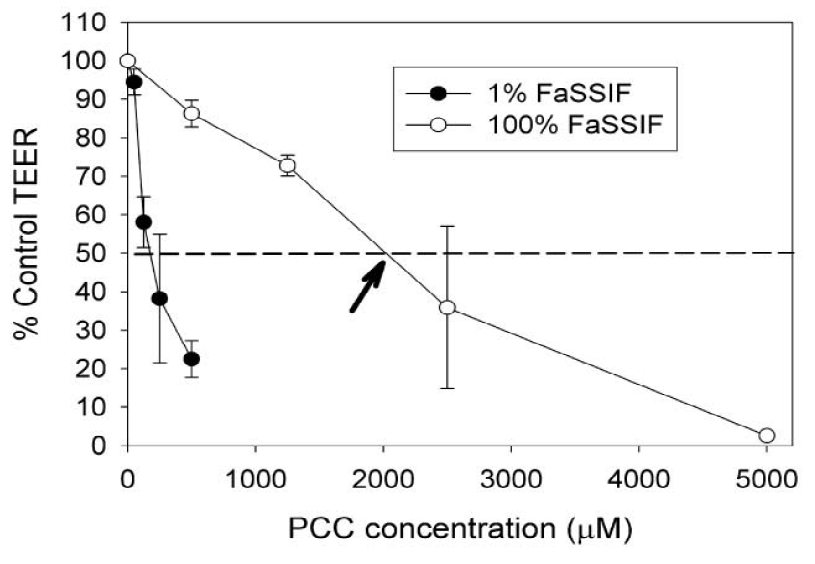
\includegraphics[width=\textwidth,height=\textheight,keepaspectratio]{graphics/devel_Fasssif_PCC3.png}
\caption{Single figure copied from \cite{tippin2008biorelevant,nawroth2011liposome} to illustrate why the potency of lipophilic permeation enhancers are likely overestimated in in-vitro studies using surfactant free buffers. Palmitoyl carnitine was found by Tippin \textit{et al} to be 12 times less potent in a Fassif buffer with Taurocholate and lechitine an EC$_{50}$}
\label{devel_fassif}
\end{figure}


\subsection{Molecular descriptors, model complexity and surfactant characteristics}
\label{modelMolecules}

\section{orphan figures}




\begin{figure}[!htbp]
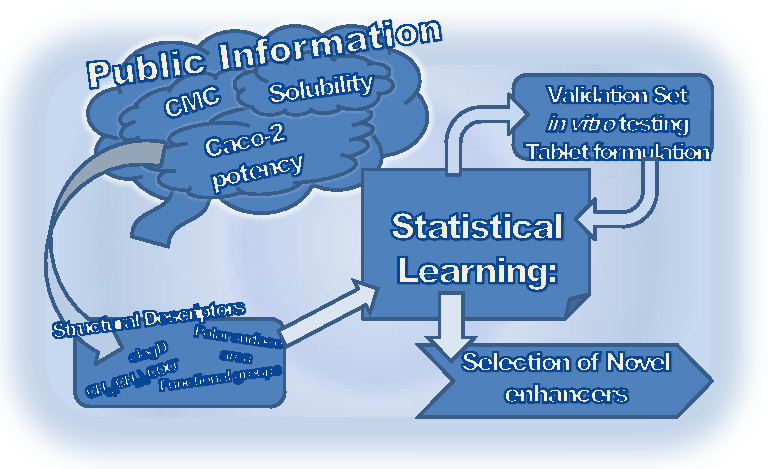
\includegraphics{graphics/workSummary_130mm.pdf}
\caption{Project idea. This figure was first designed for PhD-related presentations given by the author.}
\label{workSummary}
\end{figure}

\begin{figure}[!htpb]
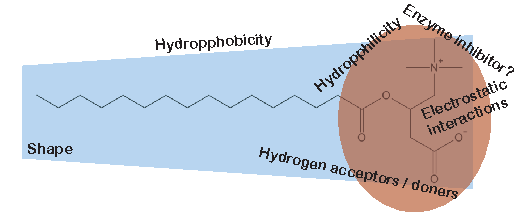
\includegraphics{graphics/typeOfSurfactant.pdf}
\caption{how does a surfactant like enhancer look like. This figure was first designed for PhD-related presentations given by the author.}
\label{typeOfSurfactant}
\end{figure}

\begin{figure}[!htpb]
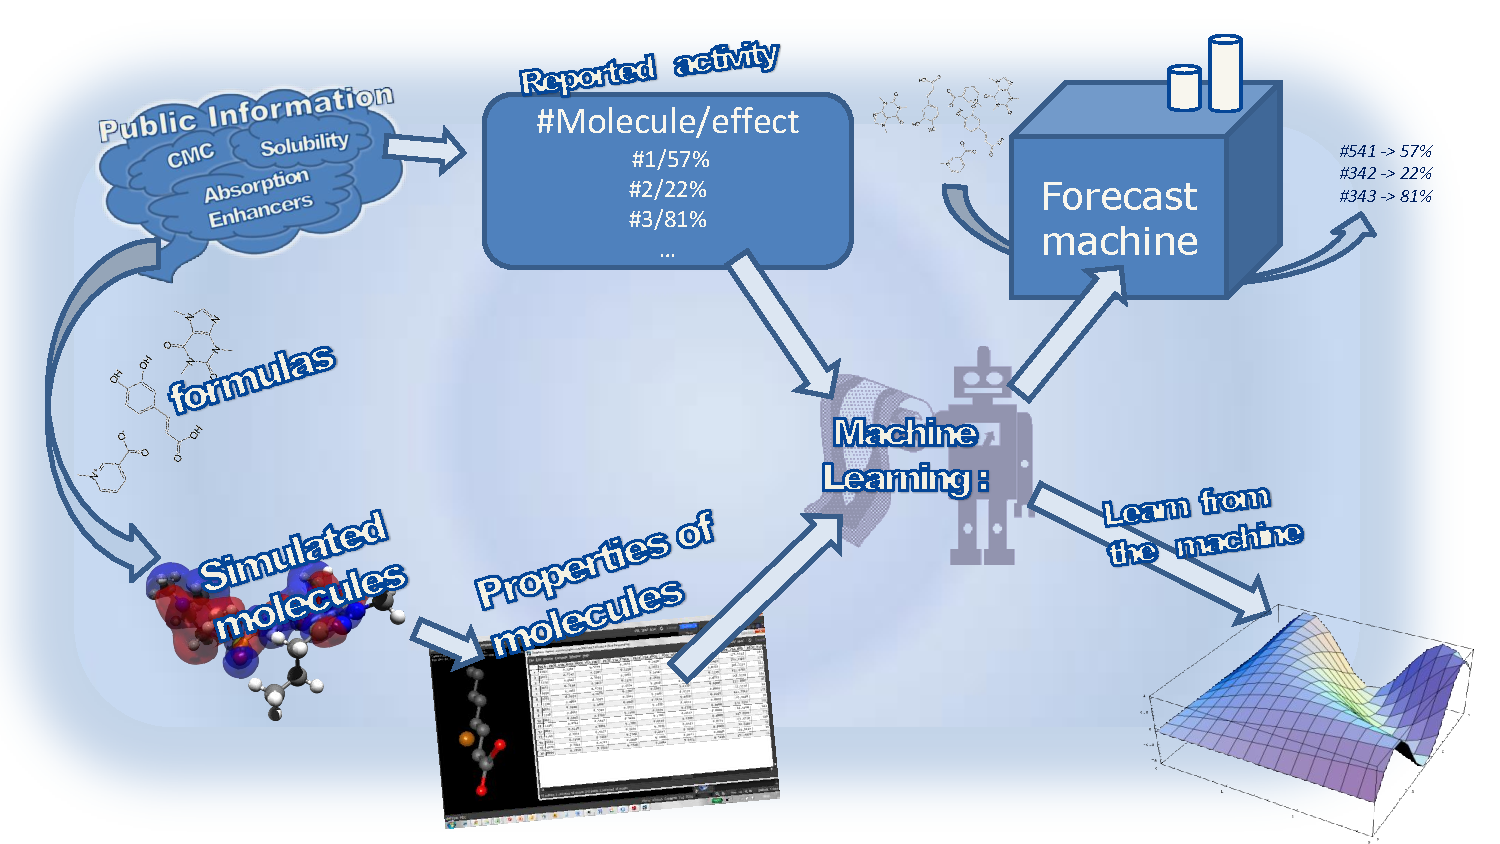
\includegraphics[width=\textwidth, height=\textheight, keepaspectratio]{graphics/predictPotencySummary.pdf}
\caption{Outline how to predictions are made. This figure was first designed for PhD-related presentations given by the author.}
\label{predictPotencySummary}
\end{figure}

The decision tree ensemble random forest have a series of useful diagnostics which have been used in this thesis work.

\section{Article: In silico modelling of permeation enhancement potency in Caco-2
monolayers based on molecular descriptors and random forest}
\label{article:predAbs}

\newpage

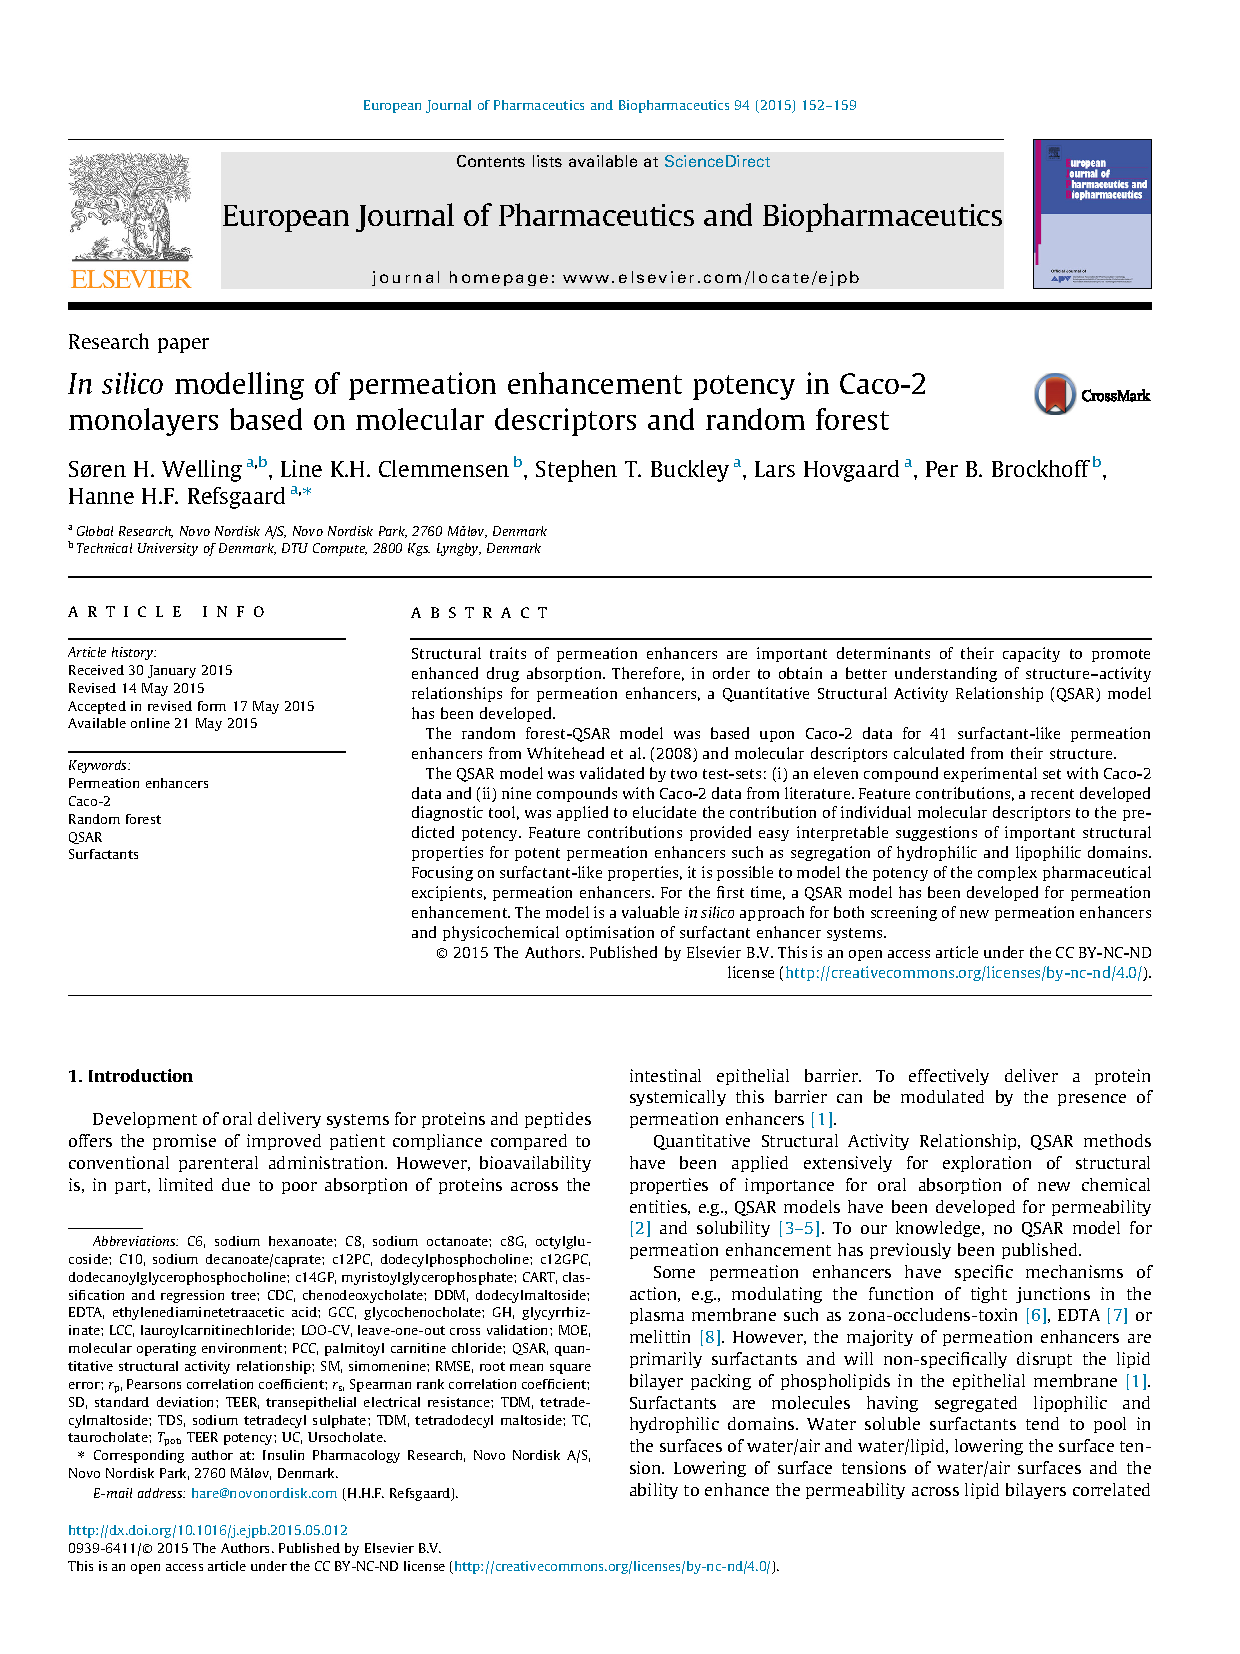
\includepdf[pages={1-},scale=0.90,pagecommand={\pagestyle{myruled}}]{chapters/predictPotencyArt.pdf}


